% !TeX program = xelatex
% !TeX encoding = UTF-8
\documentclass[journal]{IEEEtran}

\usepackage{amsmath,amssymb,mathtools}
\usepackage{booktabs,array,multirow}
\newcolumntype{C}[1]{>{\centering\arraybackslash}m{#1}}
\usepackage{graphicx}
\usepackage{newtxtext,newtxmath}
\usepackage{enumitem}
\usepackage{placeins}
\usepackage{dblfloatfix}

\usepackage[expansion=false]{microtype}
\usepackage{xurl}
\usepackage{xcolor}
\definecolor{TASECiteBlue}{HTML}{0072B2}
\usepackage[colorlinks=true,citecolor=TASECiteBlue,linkcolor=TASECiteBlue,urlcolor=TASECiteBlue]{hyperref}
\hypersetup{pdfauthor={},pdftitle={Coordinated Scheduling and Process-Mode Selection},pdfsubject={},pdfkeywords={}}
\graphicspath{{figures/}}
\setlength{\emergencystretch}{3em}
\setcounter{topnumber}{2}
\setcounter{dbltopnumber}{2}
\setcounter{dblbotnumber}{1}
\renewcommand{\topfraction}{0.90}
\renewcommand{\dbltopfraction}{0.90}
\renewcommand{\textfraction}{0.10}
\renewcommand{\floatpagefraction}{0.90}
\renewcommand{\dblfloatpagefraction}{0.95}


\usepackage{cite}

\newcommand{\method}{RDMCT-HBS}
\newcommand{\cmax}{C_{\max}}
\newcommand{\pdi}{\mathrm{PDI}}
\newcounter{algorithm}
\newcommand{\algorithmtitle}[1]{\refstepcounter{algorithm}\noindent\textbf{Algorithm~\thealgorithm: #1}\par\smallskip}

\begin{document}
\raggedbottom
\interdisplaylinepenalty=2500
\title{Coordinated Scheduling and Process-Mode Selection for Dual-Source Rotating-Chamber Cluster Tools}
\author{}
\maketitle
\begin{abstract}
Finite-batch scheduling of rotating-chamber cluster tools requires coordination of product supply, reusable dummy wafers, and periodic cleaning. This paper develops a mixed-integer linear programming model for dual-source mixed flows under full-occupancy, residency, and shared-resource constraints. A makespan-first second stage refines waiting and processing cadence within the first-stage bound. Structure-preserving initial schedules and role-aware hierarchical cut selection support time-limited solution. Computational mode comparisons use prescribed wafer-pair layouts and equal cumulative nominal processing times. The preferred mode changes with lot size and cleaning-induced chain segmentation; for 16 wafers without activated cleaning, chained processing reduces product-return makespan by 4.87\% relative to parallel processing. On the frozen algorithm benchmark, equal-budget two-stage optimization reduces total route wait by 51.91\%, while precomputed initial schedules increase incumbent availability from 51.67\% to 100\% during the subsequent solve. The learned cut selector and its hierarchical baseline have similar observed performance without a statistically established difference. These results support conditional process-mode comparison and coordinated event scheduling; physical recipe equivalence and production deployment are not established by the computational experiments.
\end{abstract}

{\small\noindent\textit{Note to Practitioners}---Engineers operating semiconductor cluster tools must coordinate production wafers with reusable dummy wafers that occupy otherwise empty positions and support chamber cleaning. A faster chamber cycle does not necessarily finish a finite lot sooner: dummy returns, robot access, and the point at which cleaning interrupts a processing chain can change the preferred operating mode. The proposed scheduler takes qualified recipes, equipment capacities, action durations, a wafer-pair layout, and available dummy inventory as inputs. It returns timed handling, processing, and cleaning actions, and can refine waiting after obtaining a feasible completion-time bound. Its intended use is offline evaluation of operating alternatives and preparation of candidate schedules. Application requires checking the input timings and occupancy rules against the actual tool and validating the resulting actions with the equipment control system. The reported tests use deterministic computational instances; they do not demonstrate film-quality equivalence, disturbance recovery, or production-line deployment. Initial-schedule construction also consumes time outside the reported main-solver budget. Users with a strict decision deadline should include this preparation cost and retain a validated fallback schedule.\par}


\begin{IEEEkeywords}
semiconductor manufacturing system , cluster tool , dual-source material flow ,
operational decision , mixed-integer linear programming , learning-enhanced exact optimization
\end{IEEEkeywords}


\section{Introduction}
Cluster tools coordinate processing modules, robots and load locks in semiconductor fabrication. Residency limits, shared handling resources and cleaning couple wafer routes and production output \cite{pan2018survey}. Multi-space modules and multi-finger robots add parallel processing and paired handling opportunities \cite{gu2024applied,gu2024multifinger}. This paper studies finite batches in plasma-enhanced chemical vapor deposition (PECVD) equipment with two four-position rotating chambers.

\begin{figure*}[t]
\centering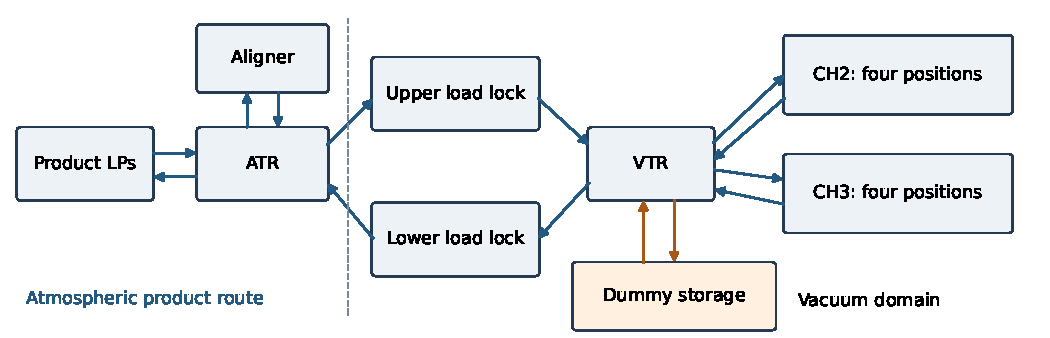
\includegraphics[width=0.94\textwidth]{fig_system_tase}
\caption{Dual-source rotating-chamber tool and product/dummy routes.}
\label{fig:system-en-new}
\end{figure*}

Products enter from atmospheric load ports; reusable dummy wafers enter from vacuum storage. Under the prescribed full-occupancy recipe, dummies fill unused positions and occupy chambers during cleaning. Their return times constrain subsequent product processing. We call these separate supplies dual-source operation, and their interleaved use of robots and chambers mixed flow. The scheduler must jointly determine product and dummy movements, robot service order, and the timing of complete processing and cleaning chains.

Two qualified processing modes are compared conditionally: $4\times1$ processes four wafers once, whereas $2\times2$ alternates paired exchanges so that every product receives two consecutive exposures. Equal cumulative nominal process time allows a scheduling comparison; it does not establish physical recipe equivalence. Cycle counts and chain initialization/termination can move cleaning inside or after the product-processing horizon. Consequently, the mode with the shortest individual cycle need not complete the lot first.

Prior work develops throughput analysis, residency-constrained linear programming and timed Petri-net models \cite{perkinson1994throughput,rostami2002optimal,wu2010closedform,qiao2012sojourn}. Extensions include revisiting routes, multiple wafer types, selectable modules and joint release/handling decisions \cite{qiao2014revisiting,wang2020multiple,wang2025virtualcell,yang2025miptwowafers}. Cleaning-aware models coordinate task sequences, wafer delay and cleaning triggers \cite{kim2013cleaning,yu2020delay,qiao2022binary,li2022conditioncleaning}. Recent T-ASE work addresses failure-related scheduling and noncyclic reinforcement-learning control \cite{zhu2025failuredeadlock,kim2025noncyclicdeadlock,kim2025adaptivecluster}. These studies motivate coordinated automation, but their schedules cannot be transferred unchanged to the present dual-source routes and rotating-chamber occupancy rules.

Learning can also assist mathematical optimization through cut ranking or selection \cite{tang2020cut,huang2022cutranking,paulus2022looking}. The hierarchical sequence model (HEM) chooses the number and ordered subset of cuts \cite{wang2023hem}. Here, mathematical variable roles augment that representation while the MILP retains responsibility for process feasibility. Numerical comparisons include HEM, configured SCIP, adaptive cut scoring and component ablations on identical models.

The contributions are: 1) a joint finite-batch model of product/dummy logistics, full occupancy, periodic cleaning and shared-resource timing under prescribed pair layouts; 2) makespan-first timing refinement and bound-based identification of how cleaning-induced chain segmentation changes mode preference; and 3) a solver framework combining structure-preserving binary-skeleton (SPBS) initialization and role-aware cut selection, with separate evidence for initialization, timing quality and search performance. The experiments support SPBS and timing refinement benefits; they do not establish statistically significant superiority of the complete learned selector over HEM.

\section{Problem description and two-stage scheduling model}


\subsection{Equipment configuration and scheduling task}

Given the product lot, process modes, wafer-pair layout, and initial equipment state, scheduling determines the start and finish times of loading, alignment, handling, rotation, processing, cleaning, and return actions, together with their order on shared resources. Products depart from LPs and return after processing. Dummies leave vacuum storage, perform filling or cleaning tasks, and return. Robot service, chamber occupancy, and dummy inventory couple the routes.

Inputs comprise action durations, resource capacities, residency limits, cleaning intervals, and dummy counts. Stage one minimizes the final product return time. Stage two improves waiting and cadence under the resulting makespan bound. Each feasible schedule is represented by an action sequence specifying wafers, resources, and start and completion times for performance evaluation and checks of precedence and resource conflicts.

Action durations are deterministic within a solve. No buffers are assumed beyond LPs, aligners, load locks, rotating chambers, and vacuum storage, so each wait corresponds to a material location and resource-occupancy interval.

\subsection{PW-pair modeling for the two process modes}

To represent wafer-level residency and paired handling together, shared transfer and chamber occupancy are modeled at the pair level, while alignment and route timing retain wafer-level events.

A wafer pair (PW pair) is a physical two-wafer transport and chamber-occupancy unit. Its members may be product+product (product PW pair), dummy+dummy (dummy PW pair), or product+dummy (mixed PW pair). Product wafers are preferentially paired by mode and index; an odd tail product may be paired with one dummy, while full-occupancy filling and cleaning may use dummy PW pairs. The sets $\mathcal P^F$ and $\mathcal P^L$ index product-containing PW pairs, including product PW pairs and any required mixed PW pairs. Alignment and residency remain wafer-level operations; the two members share a time window only on a selected two-hand transfer or the same chamber side. The prescribed layout specifies product-containing PW pairing and compatible chamber positions. The MILP optimizes the remaining activation and assignment decisions, physical dummy identities, paired transfers, resource order, and event times within this layout. Legal cleaning segments are generated from the cleaning interval and complete recipe boundaries, after which the MILP activates the cleaning tasks and schedules their times.

A product follows LP--ATR--AL--ATR--upper load lock--VTR--rotary chamber--VTR--lower load lock--ATR--LP: the ATR first places the wafer on the aligner, then retrieves it for transfer into the vacuum domain. A dummy travels from vacuum storage through the VTR to the chamber and returns through the VTR after use. A regular all-product $4\times1$ batch contains two product PW pairs, hence four product wafers, and processes all four positions synchronously once before last-in--first-out unloading; only the last incomplete batch may use a dummy or mixed PW pair to fill all positions. In $2\times2$, every product-containing PW pair occupies two adjacent process cycles so that each of its product members is processed twice. For three product PW pairs, a dummy PW pair D is loaded first, the chamber rotates, and P1 is loaded before D+P1 undergoes chamber processing. Chamber processing then alternates with ``chamber rotation + chain slide'', changing the occupancy successively to P1+P2, P2+P3, and P3+D; P1, P2, and P3 are each processed twice before all wafers are unloaded. Figures~\ref{fig:chain-en} and \ref{fig:parallel-en} show the event sequences.

\begin{figure}[t]
\centering
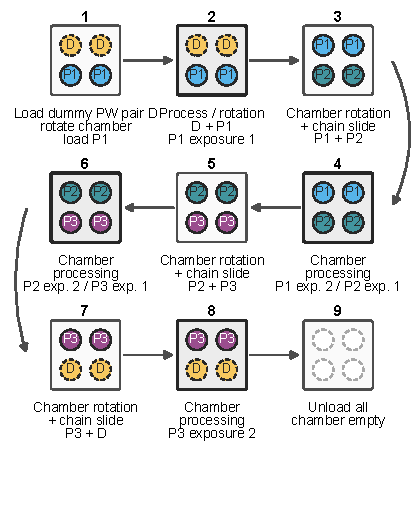
\includegraphics[width=\linewidth]{fig_chain_en_nature}
\caption{$2\times2$ chained processing. A PW pair may be P+P, D+D, or P+D; here each P$i$ is a P+P product PW pair and D is a D+D dummy PW pair. Step 1 loads D, rotates the chamber, and loads P1; Step 2 performs chamber processing on D+P1; Step 3 applies chamber rotation + chain slide to obtain P1+P2. Repeating ``chamber processing--chamber rotation + chain slide'' makes P1, P2, and P3 participate in two adjacent process cycles, so every product wafer is processed twice before all wafers are unloaded.}
\label{fig:chain-en}
\end{figure}

\begin{figure}[t]
\centering
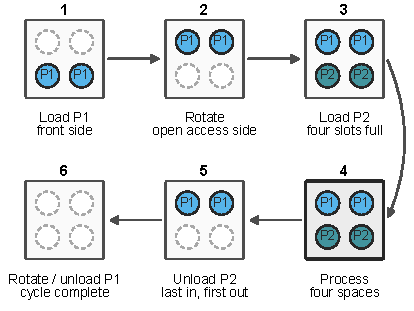
\includegraphics[width=\linewidth]{fig_parallel_en_nature}
\caption{$4\times1$ parallel processing. A regular all-product batch uses two product PW pairs, comprising four product wafers, and receives one synchronous full-occupancy process before last-in--first-out unloading; a dummy or mixed PW pair can complete the final short batch.}
\label{fig:parallel-en}
\end{figure}

The model uses chambers $c\in\mathcal C$, product wafers $w\in\mathcal W$, product-containing pairs $p\in\mathcal P^F\cup\mathcal P^L$, batch positions $b\in\mathcal B_c$, chain positions $k\in\mathcal K_c$, cycles $q\in\mathcal Q_c$, and cleaning segments $e\in\mathcal E_c$. Physical operations $o\in\mathcal O$ have start/end times $s_o,e_o$, duration $d_o$, and binary activation $b_o$. Binary $u$ denotes batch/position activation, $f$ dummy filling, $t$ or $h$ a tail, $g$ dummy assignment, $h_{o\ell}$ slot use, and $y$ resource order. Bars denote prescribed input data. $M$ is a valid horizon bound. The supplementary material provides the complete notation catalogue and expanded explanations.

\subsection{Source interfaces, operation activation, and time relations}

The fixed incidence parameter satisfies
\begin{equation}
\sum_{s\in\mathcal S}\chi_{is}=1,
\qquad i\in\mathcal I.
\label{eq:source-membership-en}
\end{equation}
If $\mathcal A^{\rm int}$ is the internal network and $\mathcal A_s$ contains release and return arcs for source $s$, then
\begin{equation}
\mathcal A=\mathcal A^{\rm int}\cup
\left(\bigcup_{s\in\mathcal S}\mathcal A_s\right).
\label{eq:route-union-en}
\end{equation}
Canonical pair positions satisfy
\begin{equation}
\begin{aligned}
x^F_{pcbl}&=\bar x^F_{pcbl}, &
\sum_{c,b,l}x^F_{pcbl}&=1 &&(p\in\mathcal P^F),\\
x^L_{pck}&=\bar x^L_{pck}, &
\sum_{c,k}x^L_{pck}&=1 &&(p\in\mathcal P^L).
\end{aligned}
\label{eq:pair-slot-en}
\end{equation}
A position containing a pair must be active, and candidate positions are used consecutively:
\begin{equation}
\begin{aligned}
x^F_{pcbl}&\le u^F_{cb}, &u^F_{c,b+1}&\le u^F_{cb},\\
x^L_{pck}&\le u^L_{ck}, &u^L_{c,k+1}&\le u^L_{ck}.
\end{aligned}
\label{eq:activation-prefix-en}
\end{equation}
For each candidate operation $o$, activation and duration satisfy
\begin{equation}
0\le s_o\le Mb_o,\qquad
0\le e_o\le Mb_o,\qquad
e_o=s_o+d_ob_o.
\label{eq:operation-time-en}
\end{equation}
For every required process arc $(o,o')\in\mathcal A$,
\begin{equation}
b_{o'}\le b_o,\qquad
s_{o'}\ge e_o+\delta_{oo'}-M(2-b_o-b_{o'}).
\label{eq:precedence-en}
\end{equation}
\subsection{Occupancy and event order in the two processing modes}

For $4\times1$, let $A^F_{cb}=\sum_{p,l}x^F_{pcbl}$ be the number of product pairs assigned to batch $(c,b)$. Full occupancy and dummy filling are
\begin{equation}
\begin{aligned}
A^F_{cb}&=\sum_{p\in\mathcal P^F}\sum_{l\in\mathcal L}x^F_{pcbl},\\
\sum_{p\in\mathcal P^F}x^F_{pcbl}+f^F_{cbl}&=u^F_{cb}
&& (l\in\mathcal L),\\
\sum_{l\in\mathcal L}f^F_{cbl}&=2u^F_{cb}-A^F_{cb}.
\end{aligned}
\label{eq:full-capacity-en}
\end{equation}
Active batches are consecutive and dummy filling is restricted to the last active batch:
\begin{equation}
\begin{aligned}
A^F_{cb}&\ge u^F_{cb}, &u^F_{c,b+1}&\le u^F_{cb},\\
A^F_{cb}&\ge2u^F_{c,b+1},
&t^F_{cb}&\le u^F_{cb},\\
t^F_{cb}&\le1-u^F_{c,b+1},
&t^F_{cb}&\ge u^F_{cb}-u^F_{c,b+1}.
\end{aligned}
\label{eq:full-tail-en}
\end{equation}
Equation~\eqref{eq:full-tail-en} requires at least one product pair in an active batch and two product pairs if a later batch is active. The last three inequalities set $t^F_{cb}=1$ exactly at the active tail; the final candidate uses $t^F_{cB}=u^F_{cB}$.

Let $FL,BL,P,BU,FU$ denote front load, back load, processing, back unload, and front unload. Then
\begin{equation}
\begin{aligned}
e^{F,\nu}_{cb}&=s^{F,\nu}_{cb}+d^{F}_{\nu}u^F_{cb}
\\[-1pt]&\nu\in\{FL,BL,P,BU,FU\},\\
s^{F,BL}_{cb}&\ge e^{F,FL}_{cb}+r_c-M(1-u^F_{cb}),\\
s^{F,P}_{cb}&=e^{F,BL}_{cb},\\
s^{F,BU}_{cb}&\ge e^{F,P}_{cb}-M(1-u^F_{cb}),\\
s^{F,FU}_{cb}&\ge e^{F,BU}_{cb}+r_c-M(1-u^F_{cb}).
\end{aligned}
\label{eq:full-sequence-en}
\end{equation}
Equation~\eqref{eq:full-sequence-en} loads the front side, rotates to load the back, starts synchronous processing after the back load, and then unloads the back side before rotating and unloading the front. Consecutive batches are linked by $s^{F,FL}_{c,b+1}\ge e^{F,FU}_{cb}-M(1-u^F_{c,b+1})$.

For $2\times2$, each product pair occupies one ordered chain position:
\begin{equation}
u^L_{ck}=\sum_{p\in\mathcal P^L}x^L_{pck},\qquad
u^L_{c,k+1}\le u^L_{ck},\qquad
a^L_c=u^L_{c1}.
\label{eq:mix-position-en}
\end{equation}
Let $q_c^-(k)$ and $q_c^+(k)$ denote the first and second process cycles of chain position $k$. The pair--cycle incidence is
\begin{equation}
\begin{aligned}
q_c^+(k)&=q_c^-(k)+1,\\
\mu^L_{pcq}
&=\sum_{\substack{k\in\mathcal K_c:\\q\in\{q_c^-(k),q_c^+(k)\}}}x^L_{pck},\\
\sum_{q\in\mathcal Q_c}\mu^L_{pcq}
&=2\sum_{k\in\mathcal K_c}x^L_{pck}.
\end{aligned}
\label{eq:mix-two-exposures-en}
\end{equation}
Equation~\eqref{eq:mix-two-exposures-en} maps every assigned $2\times2$ product-containing PW pair to exactly two adjacent process cycles. Every product member inherits the same $\mu^L_{pcq}$ incidence, so a product is not omitted even when an odd tail uses a P+D mixed PW pair. The equation also distinguishes the modes explicitly: a $2\times2$ product-containing pair spans two cycles, whereas two $4\times1$ side pairs are processed once in one full batch.

The generated layout supplies the number $\bar Q_c$ of process cycles, and $h^L_{ck}$ identifies the chain tail:
\begin{equation}
\begin{aligned}
v^L_{cq}&=
\begin{cases}a^L_c,&q\le\bar Q_c,\\0,&q>\bar Q_c,
\end{cases}\\
\sum_k h^L_{ck}&=a^L_c,\qquad
h^L_{ck}\le u^L_{ck},\qquad
h^L_{ck}+u^L_{c,k+1}\le1,\\
h^L_{ck}&\ge u^L_{ck}-u^L_{c,k+1}.
\end{aligned}
\label{eq:mix-layout-en}
\end{equation}
Equation~\eqref{eq:mix-layout-en} gives $n+1$ process cycles for a segment with $n$ product-containing PW pairs: the head is dummy PW pair+P1, internal cycles are P$i$+P$i+1$, and the tail is P$n$+dummy PW pair. The final relations make $h^L_{ck}$ one only at the last active product position.

For a legal chain segment $(q_0,\ldots,q_T)$, let $H_0$, $B_q$, and $T_0$ denote head loading, internal exchange, and tail unloading. Then
\begin{equation}
\begin{aligned}
e^L_{cq}-s^L_{cq}&=d^L v^L_{cq},\\
s^L_{cq_0}&=e^{H_0}_c,\\
s^{B}_{cq}&\ge e^L_{c,q-1}-M(1-a^L_c),\\
s^L_{cq}=e^{B}_{cq}\quad(q_0<q\le q_T),\\
s^{T_0}_c&\ge e^L_{cq_T}-M(1-a^L_c).
\end{aligned}
\label{eq:mix-sequence-en}
\end{equation}
Equation~\eqref{eq:mix-sequence-en} begins the first process immediately after head loading, performs an internal exchange only after the previous cycle, and unloads the tail only after the last process. It directly realizes dummy+P1, P1+P2, $\ldots$, Pn+dummy.

\subsection{Cleaning and reusable dummy wafers}

Cleaning segments are generated from $H$ and complete process boundaries and enter the MILP as fixed binary indicators:
\begin{equation}
z_{ce}=\bar z_{ce},\qquad
a^F_{cbe}=\bar a^F_{cbe}u^F_{cb},\qquad
a^L_{cqe}=\bar a^L_{cqe}v^L_{cq}.
\label{eq:clean-layout-en}
\end{equation}
Equation~\eqref{eq:clean-layout-en} prevents arbitrary cleaning locations: $4\times1$ may split only at batch boundaries and $2\times2$ only after a complete chain segment, while the MILP still schedules process and cleaning times.

Let $N_{ce}$ be the number of active process cycles in segment $e$:
\begin{equation}
\begin{gathered}
N_{ce}=\sum_b a^F_{cbe}+\sum_q a^L_{cqe},\qquad
z_{ce}\le N_{ce}\le Hz_{ce},\\
q^{\rm cl}_{ce}=z_{c,e+1}+\tau_{ce},\qquad z_{c,E_c+1}=0.
\end{gathered}
\label{eq:clean-count-en}
\end{equation}
Equation~\eqref{eq:clean-count-en} places at least one and at most $H$ process cycles in an active segment. It activates an internal cleaning before every subsequent production segment and, when the final segment exactly exhausts $H$ cycles, sets $\tau_{ce}=1$ to activate terminal cleaning. Both are complete equipment actions; only the terminal action has no subsequent product processing.

Let $\mathcal V_c$ be the union of $4\times1$ batches and $2\times2$ cycles and let $a_{vce}$ take the corresponding $a^F$ or $a^L$. Cleaning order and the physical cleaning chain satisfy
\begin{equation}
\begin{aligned}
s_v&\ge e^{\rm cl}_{c,e-1}-M(1-a_{vce}) &&(e>1),\\
e_v&\le s^{\rm cl}_{ce}+M(1-a_{vce})+M(1-q^{\rm cl}_{ce}),\\
s^{\rm cl,BL}_{ce}&\ge e^{\rm cl,FL}_{ce}+r_c-M(1-q^{\rm cl}_{ce}),\\
s^{\rm cl,P}_{ce}&\ge e^{\rm cl,BL}_{ce}-M(1-q^{\rm cl}_{ce}),\\
s^{\rm cl,BU}_{ce}&\ge e^{\rm cl,P}_{ce}-M(1-q^{\rm cl}_{ce}),\\
s^{\rm cl,FU}_{ce}&\ge e^{\rm cl,BU}_{ce}+r_c-M(1-q^{\rm cl}_{ce}).
\end{aligned}
\label{eq:clean-time-en}
\end{equation}
Equation~\eqref{eq:clean-time-en} starts a segment after the preceding cleaning and finishes it before the next cleaning. A cleaning task loads both chamber sides with dummies, rotates, processes, and unloads in reverse, thereby occupying the VTR, chamber, and four physical dummies rather than adding virtual downtime.

Dummy demand $j$ is activated by a physical event:
\begin{equation}
q_j=
\begin{cases}
f^F_{cbl},&j\text{ is a final-$4\times1$ filling demand},\\
a^L_c,&j\text{ is a chain endpoint demand},\\
q^{\rm cl}_{ch},&j\text{ is a cleaning demand}.
\end{cases}
\label{eq:dummy-demand-en}
\end{equation}
Equation~\eqref{eq:dummy-demand-en} prevents dummies from becoming an unlimited abstract filler: a physical demand exists only for a final batch, chain head/tail, or active cleaning task.

Each active demand selects one physical dummy from inventory:
\begin{equation}
\sum_{\tau\in\mathcal T_c}g_{j\tau}=q_j,
\qquad j\in\mathcal J_c^D.
\label{eq:dummy-assign-en}
\end{equation}
\subsection{Robots, load locks, chambers, and time resources}

ATR, AL, VTR, and each rotary chamber are unary resources; the upper and lower load locks each have two physical slots; each dummy in inventory is a reusable slot. An operation $o$ requiring $\kappa_o$ slots satisfies
\begin{equation}
\sum_{\ell\in\Gamma_o}h_{o\ell}=\kappa_ob_o.
\label{eq:slot-select-en}
\end{equation}
If operations $o$ and $o'$ may compete for slot $\ell$ of resource $r$, then
\begin{equation}
\begin{aligned}
s_{o'}&\ge e_o+\rho^r_{oo'}-M(1-y^r_{oo'})
-M(1-h_{o\ell})-M(1-h_{o'\ell}),\\
s_o&\ge e_{o'}+\rho^r_{o'o}-My^r_{oo'}
-M(1-h_{o\ell})-M(1-h_{o'\ell}).
\end{aligned}
\label{eq:resource-order-en}
\end{equation}
Equation~\eqref{eq:resource-order-en} makes $y^r_{oo'}$ choose one order whenever two actions use the same slot and includes empty robot travel or equipment reset through $\rho^r_{oo'}$. It applies to ATR, AL, both load locks, VTR, rotary chambers, and individual dummies, preventing concurrent robot actions and reuse before release.

An individual product or dummy stage must coincide with its selected batch, chain position, or cleaning window. For selection $x$ and reference stage $[s^{\rm ref},e^{\rm ref}]$,
\begin{equation}
\begin{aligned}
-M(1-x)&\le s_o-s^{\rm ref}\le M(1-x),\\
-M(1-x)&\le e_o-e^{\rm ref}\le M(1-x).
\end{aligned}
\label{eq:stage-link-en}
\end{equation}
If pair $p$ uses one paired transfer on robot route $a$, the two wafer stages are synchronized:
\begin{equation}
\begin{aligned}
-M(1-\gamma_{pa})&\le s_{w_1a}-s_{w_2a}\le M(1-\gamma_{pa}),\\
-M(1-\gamma_{pa})&\le e_{w_1a}-e_{w_2a}\le M(1-\gamma_{pa}).
\end{aligned}
\label{eq:double-transfer-en}
\end{equation}
For the entry and exit events of wafer $w$ in restricted equipment region $r$,
\begin{equation}
0\le s_{\operatorname{out}(w,r)}-e_{\operatorname{in}(w,r)}
\le\overline R_{wr}.
\label{eq:residence-en}
\end{equation}
Equation~\eqref{eq:residence-en} limits the physical stay in an upper load lock, chamber, lower load lock, or restricted transport region. Load-lock occupation also spans placement, pump/vent, opposite-side pickup, and pressure reset, so placement by a robot is not mistaken for slot release.

\subsection{Makespan-first two-stage optimization}

Let $C_w$ be the time at which product wafer $w$ completes the lower-load-lock return and reaches its load port. Stage one solves
\begin{equation}
C_w=e_{w,\mathrm{return}},\qquad
C_{\max}\ge C_w\ (w\in\mathcal W),\qquad
\min_{\xi\in\mathcal F}C_{\max}.
\label{eq:primary-objective-en}
\end{equation}
Equation~\eqref{eq:primary-objective-en} measures makespan at the last product wafer's return to LP after its complete end-to-end route. Internal cleaning affects $C_{\max}$ through resource occupancy and precedence that delay subsequent product returns. Terminal cleaning remains in the action sequence, but its completion time does not directly lower-bound $C_{\max}$. It can still affect other chambers' product returns through competition for the shared VTR; this indirect effect is determined by the complete schedule. WPH uses product-return makespan as its denominator. The feasible region $\mathcal F$ is defined by Eqs.~\eqref{eq:source-membership-en}--\eqref{eq:residence-en} expanded over all applicable indices.

Given stage-one incumbent $\widehat\xi$ and makespan $\widehat C$, stage two fixes the discrete structure indexed by $\mathcal D_{\rm fix}$ and minimizes linear schedule quality within the makespan tolerance:
\begin{equation}
\begin{gathered}
\xi_d=\widehat\xi_d\quad(d\in\mathcal D_{\rm fix}),\qquad
C_{\max}\le\widehat C+\varepsilon_C,\\
L_{\rm sum}=\sum_{\alpha\in\mathcal Q^w}\omega_\alpha,\qquad
L_{\max}\ge\omega_\alpha,\\
\Delta_{ceq}=(h_{ce,q+1}-h_{ceq})-(h_{ceq}-h_{ce,q-1}),\\
v_{ceq}\ge\Delta_{ceq},\qquad v_{ceq}\ge-\Delta_{ceq},\\
\eta_\alpha\ge\omega_\alpha-\bar\omega_\alpha,\qquad
\eta_\alpha\ge0,\\
\min\Phi=\lambda_1L_{\rm sum}+\lambda_2L_{\max}
+\lambda_3\sum_{(c,e,q)\in\mathcal I_h}v_{ceq}
+\lambda_4\sum_{\alpha\in\mathcal Q^w}\eta_\alpha.
\end{gathered}
\label{eq:secondary-objective-en}
\end{equation}
Equation~\eqref{eq:secondary-objective-en} preserves the stage-one makespan bound and fixes the principal discrete routes and resource orders. Retained paired-transfer choices and continuous times can change to reduce total wait, maximum wait, and variation between consecutive processing intervals within each segment. Optional soft-limit excess can also be penalized. The experiments use $(\lambda_1,\lambda_2,\lambda_3)=(1,10,25)$ and $\varepsilon_C=10^{-6}$. With the soft waiting limit disabled, no excess variables are generated. For a time-limited first stage, the best incumbent value $\widehat C$ supplies the second-stage bound; variables in $\mathcal D_{\rm fix}$ are fixed while designated paired-transfer variables remain adjustable.

\section{Structure-Aware Solution Framework}
\label{sec:method-new}
SCIP generates valid inequalities, checks incumbents and maintains primal/dual bounds \cite{achterberg2009scip,bestuzheva2023scip}. SPBS provides an initial feasible schedule and \method{} selects from solver-generated cuts. Neither component changes the model's integer feasible set. The supplementary material gives the expanded network, feature and training definitions.

\subsection{SPBS initial solution}
SPBS constructs a conservative discrete schedule from the recipe and tool layout. Products are paired in input order; parallel-mode pairs are placed sequentially and chained-mode pairs round-robin across chambers. Complete chains determine cleaning boundaries, and deterministic load-lock slots break symmetry. ATR/VTR order follows product progression and dummy return.

A restricted MILP fixes the binary skeleton and solves for compatible event times. Five relaxation levels successively release VTR order, load-lock order, other resource orders, and slot choices, retaining prescribed structural assignments. Large instances start at less restrictive levels. Each subproblem uses a zero objective, feasibility emphasis, aggressive heuristics and no cut separation, and stops at its first feasible solution. Failure to find one within a level's budget is not an infeasibility certificate.

After completing auxiliary schedule-quality variables, a candidate must pass the original-model feasibility check before becoming an incumbent. The main solve restores original bounds. These initial schedules are precomputed in the reported benchmark; their construction cost is excluded from main-solve timing and PDI. Thus the SPBS comparison estimates the value of an available feasible start, not an initialization-inclusive speedup.

\subsection{Role-aware hierarchical cut selection}
The 2023 HEM sequence model is the direct learned baseline \cite{wang2023hem}; its later sequence/set extension is related work \cite{wang2024hemset}. The 13 baseline features measure objective parallelism, efficacy, support, integral support, violation, and four statistics each of cut and objective coefficients. Ten added features describe five variable-role coefficient masses, finite-bound mass, positive-coefficient mass, discrete--continuous coupling, dominant-role mass and role entropy. Roles are binary, general integer, objective-active continuous, other continuous auxiliary, and residual variables. For cut coefficients $a_{ij}$, role mass is
\begin{equation}
p_{ig}=\frac{\sum_{j:x_j\in g}|a_{ij}|}{\sum_j|a_{ij}|+\varepsilon}.
\end{equation}
Feature extraction uses variable type, objective coefficient and global bounds, so renaming variables leaves the representation unchanged.

After layer normalization, separate linear projections of the 13 generic and ten role features are fused with a sigmoid gate. A one-layer 128-unit LSTM encodes candidates; a pointer decoder uses one glimpse and masks previously selected rows \cite{vinyals2015pointer}. A high-level policy predicts the retained count. At inference, width-three beam search retains the highest accumulated log-probability prefixes \cite{choo2022beam}. Candidates are capped at 128 in efficacy order; at most 20\% and 16 rows are retained, subject to SCIP's limit. Forced cuts remain under solver control.

The first $\lceil0.25k\rceil$ decoded rows serve as fixed anchors. Greedy completion selects remaining rows from at most $2k$ policy/heuristic candidates by marginal gain of
\begin{equation}
\begin{aligned}
F(S)={}&\sum_{i\in S}(0.35q_i+0.20r_i)
+0.25\sum_g d_g\sqrt{\sum_{i\in S}p_{ig}}\\
&+\frac{0.20}{|\mathcal R|}\sum_{u\in\mathcal R}\max_{i\in S}s_{ui}.
\end{aligned}
\end{equation}
Here $q_i$ combines instantaneous cut quality and role descriptors, $r_i$ is a normalized pointer-rank prior, $d_g$ is pool role demand, and $s_{ui}$ is clipped cosine similarity. Nonnegative weights make this a monotone submodular surrogate. For fixed anchors and pool, greedy residual completion has the standard $1-1/e$ approximation property \cite{nemhauser1978analysis}; this is not a guarantee for PDI or solve time. Anchor order precedes greedy-completion order when cuts enter the LP.

\subsection{Training protocol}
Training uses five instances, five independent training seeds and the fixed epoch-60 checkpoint. Each epoch collects eight 30-s/1024-MB rollouts with two workers. The terminal PDI is the cost; the first eligible candidate-set action supplies the high/low-level log-probability sample. Parallel hierarchical REINFORCE uses separate exponential-moving-average baselines (decay 0.9), sequence-length-normalized low-level log probability, and gradient clipping at 2 \cite{williams1992reinforce,mnih2016a3c}. The high level updates every two epochs. Adam learning rates start at $10^{-4}$ and $5\times10^{-4}$ and decay by 0.96 every ten epochs. HEM, feature-only and complete policies are trained separately. Stochastic training and beam inference are distinguished; test-instance performance is not used to select checkpoints.

\section{Computational experiments and results}
\label{sec:results-new}

\subsection{Experimental design and metrics}

The experiments examine four questions: how lot size and cleaning interval affect mode preference; whether equal-budget two-stage optimization improves waiting and cadence; how SPBS and structure-aware cut selection separately affect feasible-schedule availability and primal--dual convergence; and how scale, composition, and parameter changes affect computational performance. The evidence comprises mode comparisons, the direct HEM comparison, 960 paired SPBS runs, 1500 equal-budget refinement runs, 300 factorial runs, 80 one-factor perturbation runs, and 729 distribution-shift runs across all methods on 40--64-wafer lots. Resource Gantt charts show chained-mode operation for 16 wafers at $H=10$ and $H=3$. Every feasible schedule used in the analysis passes SCIP validation against the original model and independent event-time checks.

Within each comparison family, methods share the MILP, SCIP version, instances, random seeds, time and memory limits. The algorithm benchmark uses root-only cut separation, including its configured SCIP baseline. Let $P(t)$ denote the primal bound of the minimization problem at time $t$, namely the objective value of the best incumbent, and let $D(t)$ denote the dual bound, namely the global lower bound certified by the search tree. Define $\Delta(t)=|P(t)-D(t)|$, $m(t)=\min\{|P(t)|,|D(t)|\}$, and $M(t)=\max\{|P(t)|,|D(t)|\}$. When the two bounds are finite, have the same sign, and differ, the terminal relative primal--dual gap is defined in SCIP as
\begin{equation}
G_{\rm end}=100\,\frac{\Delta(T)}{m(T)}.
\label{eq:terminal-gap-en}
\end{equation}
SCIP sets $G_{\rm end}=0$ when the bounds coincide and returns $+\infty$ when they have opposite signs or valid bounds are not both available. Equation~\eqref{eq:terminal-gap-en} normalizes by the smaller absolute bound and consequently does not cap $G_{\rm end}$ at 100\%. A value above 100\% indicates that the absolute bound difference exceeds the smaller absolute bound.

SCIP uses a different bounded normalization for the primal--dual integral. Define the instantaneous integral gap as
\begin{equation}
g_{\rm PDI}(t)=100\,\frac{\Delta(t)}{M(t)},\qquad
\pdi=\int_0^T g_{\rm PDI}(t)\,\mathrm dt.
\label{eq:pdi-gap-en}
\end{equation}
Equation~\eqref{eq:pdi-gap-en} applies when the bounds are finite, have the same sign, and differ; SCIP sets $g_{\rm PDI}(t)=0$ for coincident bounds and $g_{\rm PDI}(t)=100$ otherwise. The instantaneous integral gap is therefore bounded to $[0,100]$; lower PDI means that the bound gap closes earlier. PDI is zero only if the gap is zero for almost the entire timed horizon, whereas $G_{\rm end}=0$ only states that optimality is proved at termination. Both quantities follow SCIP definitions and use its solution statistics \cite{achterberg2009scip,bestuzheva2023scip}.

The manufacturing instance is the inferential unit: random repeats are first aggregated within an instance, after which paired instance differences use nonparametric 95\% bootstrap intervals, Wilcoxon signed-rank tests, and Holm correction within each prespecified analysis family. Time-limited runs remain in the summaries so that random seeds are not treated as independent manufacturing evidence. 

Two experiment families use different prescribed configurations. The frozen algorithm benchmark uses nominal 180-s durations for both a parallel process and each chained exposure, a 500-s module-residency bound, and $H=5$ in the nominal core suite. Its PDI and schedule-quality comparisons concern methods solving the same instances; they do not compare equal-dose process modes. The mode-selection study instead uses 180~s versus 90+90~s and a 10000-s module-residency bound. The numerical values in Table~\ref{tab:gantt-config-en} apply to the latter family. The product-return comparison uses equal cumulative nominal processing time: 180~s for one $4\times1$ exposure and 90+90~s for two $2\times2$ exposures. Recipe qualification is a prescribed input condition for this scheduling comparison.

The two chambers share the VTR. Displayed schedules pass original-model and event-time checks.

\begin{table*}[!htbp]
\centering
\footnotesize
\setlength{\tabcolsep}{2pt}
\caption{Experimental parameters for the cleaning-frequency mode experiment and representative Gantt charts under equal total nominal processing time.}
\label{tab:gantt-config-en}
\begin{tabular}{C{0.10\textwidth} C{0.29\textwidth} C{0.10\textwidth} C{0.29\textwidth}}
\toprule
Group & Parameter and value & Group & Parameter and value\\
\midrule
Rotating chambers & CH2 and CH3; two shared rotating PMs with four spaces each & Process time & 180~s for $4\times1$; 90+90~s for $2\times2$\\
Cleaning & At most $H=3$--10 effective process cycles between adjacent cleanings; pure-dummy cleaning 500~s & Chamber motion & 180$^\circ$ rotation 2~s; inter-action gap 1~s\\
ATR & One dual-hand robot, capacity 2; load/unload 4~s, complete loaded transfer 11~s & VTR & One four-hand robot, capacity 4; loaded transfer 4~s, empty reposition 4~s\\
ATR details & LL--LP empty return 6~s; PW-pair exchange at AL 8~s & AL & Capacity 1; minimum alignment occupancy 20~s per wafer\\
Load locks & LLupper pump/reset 30~s per slot; LLlower vent/reset 25~s & LL capacity & Two independent slots in each of upper and lower LLs\\
Material source & LP1--LP4, capacity 25 wafers each & Dummy wafers & Eight reusable wafers, four per chamber; storage capacity 10\\
Batch and model & Product batch size 4; 13 modeled process steps & Chamber bound & At most 15 $4\times1$ batch slots per PM\\
Model bounds & Big-$M=10000$; module and robot residency bounds 10000~s & Waiting option & Avoidable-wait hard cap 0, meaning that this optional cap is disabled\\
Objective & Product-return makespan and waiting refinement & Policy & Fixed training seed 1, epoch 60, 23 features\\
Decoder and cuts & Beam width 3; cut pool 128, at most 16 cuts selected per round & Solver & SCIP seed 1; Available, validated initial schedules\\
Solve and selection & Product-return objective; makespan bounds for mode comparison; waiting-refined schedules for Gantt charts & Schedule validation & Original-model and independent validation for every schedule\\
\bottomrule
\end{tabular}
\end{table*}

\subsection{Process-mode selection driven by cleaning position and lot size}

Steady-state analyses of multi-space CTs usually measure cycle time or throughput \cite{gu2024multifinger}. For finite batches, we define $C_{\max}$ as the time when the last product wafer returns to an LP and define equivalent batch output as $\mathrm{WPH}=3600|\mathcal W|/C_{\max}$. Pure $4\times1$ uses 180~s per wafer, pure $2\times2$ uses 90+90~s, and a 1:1 mixture assigns each product its mode-specific recipe. The cleaning interval $H$ counts full-occupancy cycles per chamber: a $4\times1$ batch counts once and each $2\times2$ exposure counts separately. Processing segments follow cycle limits and complete-chain boundaries, including 500-s cleaning and associated dummy loading, unloading, rotation, and transport.

Table~\ref{tab:clean-crossover-en} gives the $H=3$--10 comparison. The $H=4$--9 experiment contains 36 configurations with training and solver seeds fixed at 1, a 14400-s main-solve limit, and stage~2 disabled. All 36 schedules pass independent validation; 35 are proven optimal. For 16 wafers at $H=5$, pure $2\times2$ reaches a feasible 907~s within that budget. A separate 28800-s solve of the same instance, initialized from this schedule, improves the upper bound to 898~s, with lower bound 694~s and terminal gap 29.39\%. The improved schedule passes main-model and 4-s exchange checks. This extended-budget experiment determines the feasible upper bound used for mode comparison; its computation time is excluded from the fixed-budget algorithm comparison. With cleaning inactive, the 16-wafer pure $2\times2$ models at $H=6$--10 are identical and have optimum 898~s.


\begin{table*}[tp]
\centering
\footnotesize
\setlength{\tabcolsep}{3pt}
\caption{Makespans, cleaning counts, and preferred modes under the prescribed PW layouts for 8-, 16-, and 24-wafer lots at $H=3$--10. Times are in seconds.}
\label{tab:clean-crossover-en}
\begin{tabular}{cccccccccc}
\toprule
\multirow{2}{*}{Lot (wafers)} & \multirow{2}{*}{$H$} & \multicolumn{3}{c}{$C_{\max}$ (s)} & \multirow{2}{*}{$\Delta C_{\max}$ (s)} & \multicolumn{3}{c}{Total cleans} & \multirow{2}{*}{Preferred mode}\\
\cmidrule(lr){3-5}\cmidrule(lr){7-9}
 & & Pure $4\times1$ & Pure $2\times2$ & 1:1 mixed & & Pure $4\times1$ & Pure $2\times2$ & 1:1 mixed & \\
\midrule
8 & 3 & 610 & 578 & 654 & -32 & 0 & 2 & 1 & Pure $2\times2$\\
8 & 4--10 & 610 & 578 & 654 & -32 & 0 & 0 & 0 & Pure $2\times2$\\
\midrule
16 & 3 & 944 & 1402 & 1530 & 458 & 0 & 4 & 2 & Pure $4\times1$\\
16 & 4 & 944 & 1470 & 939 & 526 & 0 & 2 & 2 & 1:1 mixed\\
16 & 5 & 944 & 898$^{\dagger}$ & 939 & -46 & 0 & 2 & 0 & Pure $2\times2$\\
16 & 6--10 & 944 & 898 & 939 & -46 & 0 & 0 & 0 & Pure $2\times2$\\
\midrule
24 & 3 & 1268 & 2220$^{\dagger}$ & 2324$^{\dagger}$ & 952 & 2 & 6 & 4 & Pure $4\times1$\\
24 & 4 & 1268 & 2928$^{\dagger}$ & 1827$^{\dagger}$ & 1660 & 0 & 4 & 2 & Pure $4\times1$\\
24 & 5 & 1268 & 1769$^{\dagger}$ & 1796 & 501 & 0 & 2 & 2 & Pure $4\times1$\\
24 & 6 & 1268 & 1880$^{\dagger}$ & 1263$^{\dagger}$ & 612 & 0 & 2 & 1 & 1:1 mixed\\
24 & 7 & 1268 & 1237$^{\dagger}$ & 1250 & -31 & 0 & 2 & 0 & Pure $2\times2$\\
24 & 8--10 & 1268 & 1237$^{\dagger}$ & 1250 & -31 & 0 & 0 & 0 & Pure $2\times2$\\
\bottomrule
\end{tabular}
\par\smallskip
\parbox{0.95\textwidth}{\footnotesize Cleaning counts sum internal and terminal cleans across both chambers. $\dagger$ denotes a feasible upper bound; other times are proven optima. $\Delta C_{\max}$ subtracts the listed pure $4\times1$ time from the pure $2\times2$ time. A preferred mode is established by comparing optima or by a feasible upper bound below the competing lower bounds.}
\end{table*}

For 8 wafers, chained processing is preferred throughout $H=3$--10. For 16 wafers, parallel, mixed and chained modes are preferred at $H=3$, $H=4$, and $H=5$--10, respectively. At $H=5$, the validated 898-s chained schedule beats both competing optima even though its own optimality is unresolved. At $H=6$--10, 898~s is proven optimal, 4.87\% below parallel operation.

The 16-wafer chained layout contains four product pairs per chamber. It splits them as 2+2 at $H=3$, 3+1 at $H=4$, and one chain at $H\ge5$. Equal internal-cleaning counts at $H=3$ and 4 therefore need not give equal makespans. The study compares the joint effect of the cleaning limit and regenerated admissible chain layout.

The 24-wafer extension covers all three modes at $H=3$--6 with 7200~s per configuration. Pure $4\times1$ has optimum 1268~s at each interval. At $H=4$, pure $2\times2$ and mixed-mode lower bounds are 1342 and 1774~s; at $H=5$, the pure $2\times2$ lower bound is 1440~s and the mixed optimum is 1796~s. These bounds establish pure $4\times1$ as preferred at both intervals. At $H=6$, the mixed-mode upper bound of 1263~s is below the pure $4\times1$ optimum and pure $2\times2$ lower bound of 1440~s, establishing mixed-mode dominance; its terminal gap is 10.40\%. At $H=3$, a 28800-s solve for pure $2\times2$ obtains a validated 2220-s schedule, lower bound 2082~s, and gap 6.63\%. This lower bound and the mixed-mode lower bound of 2302~s exceed the pure $4\times1$ optimum. The extended-budget solve determines mode ordering; its computation time is excluded from the fixed-budget algorithm comparison. Hence pure $4\times1$ is preferred for 24 wafers at $H=3$--5 and mixed operation at $H=6$. The difference from the 16-wafer $H=5$ result demonstrates the dependence on lot size and complete-chain layout.

All 12 configurations in the 24-wafer $H=7$--10 extension yield validated schedules. An independent solve for mixed operation at $H=10$ proves a makespan of 1250~s within the 28800-s budget. The mixed-mode MILPs at $H=7$--10 have identical objectives, constraints, and variable bounds, so all four intervals have the same optimal makespan. Pure $2\times2$ yields a feasible 1237-s schedule at $H=8$--10. Transferring its production-event timing to the $H=7$ model and scheduling two terminal cleanings also gives a 1237-s schedule that passes validation against the original model. The valid pure $2\times2$ intervals are $[712,1237]$~s at $H=7$ and $[842,1237]$~s at $H=8$--10. These upper bounds are below the mixed-mode optimum of 1250~s and pure $4\times1$ optimum of 1268~s. Thus, pure $2\times2$ is preferred throughout $H=7$--10, with the constructed schedules reducing makespan by 1.04\% and 2.44\%, respectively. Extended-solve and schedule-transfer costs are accounted for separately from the fixed-budget algorithm comparison.

The resource Gantt charts show 16-wafer chained operation at $H=10$ and 3. To study waiting at minimum makespan, the $H=10$ pure $2\times2$ schedule is further optimized for total route wait under $C_{\max}\le898+10^{-6}$~s, with resource order allowed to change. The minimum route wait is 492~s, accumulated over six consecutive-operation intervals for each product wafer: 448~s from AL pair coordination, 36~s before post-processing unloading, and 8~s before return from the lower load lock. This route measure is distinct from the interval between consecutive in-chamber exposures. Each time axis ends at the last product return, $C_{\max}$. Every pure $4\times1$ process lasts 180~s and every pure $2\times2$ exposure lasts 90~s.

Chamber lanes distinguish gray exchange actions from pale-pink waiting. A combined exchange by the four-finger VTR takes 4~s. A split exchange includes 4-s unloading, at least 4~s of empty repositioning, and 4-s loading; other material actions may be coordinated between unloading and loading. In Fig.~\ref{fig:gantt-cleanH10-22-en}, the first CH2 inter-exposure interval is 63~s: 59~s waiting followed by a 4-s combined exchange. The next product PW, W5/W6, enters the upper load lock at 299~s and completes vacuum-side preparation at 329~s. CH2 finishes processing at 270~s, waits until 329~s, and exchanges at 329--333~s. Most adjacent cycles in the $H=3$ short-chain schedule use continuous 4-s combined exchanges; CH2 cycles five and six are separated by waits at 1106--1108~s and 1112--1116~s, unloading at 1108--1112~s, and loading at 1116--1120~s. The final exposure starts immediately at 1120~s and ends at 1210~s. Every exposure remains 90~s. Constraining all eight inter-exposure intervals in the same $H=10$ model to exactly 4~s yields an independently validated optimum of 960~s, 62~s (6.90\%) above 898~s. Continuous exchanges compress local intervals but restrict supply and return order on shared resources; allowing local waiting shortens this finite batch's makespan.



\begin{figure*}[!t]
\centering
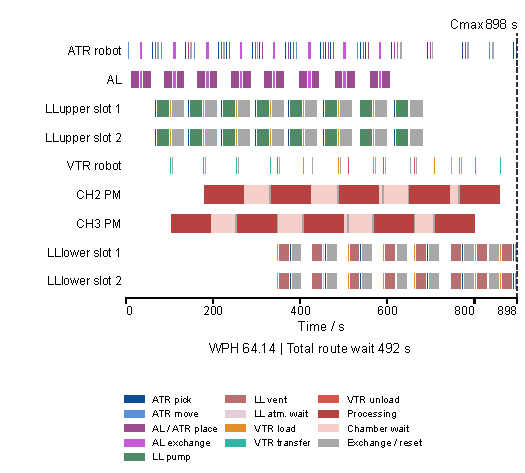
\includegraphics[width=0.825\textwidth]{fig_resource_gantt_cleanH10_w16_22_en_nature}
\caption{16-wafer pure $2\times2$ schedule at $H=10$, without cleaning: $C_{\max}=898$~s, WPH = 64.14 wafers/h. Refinement minimizes total route wait to 492~s at this makespan. Gray denotes 4-s chamber exchanges; pale pink denotes waiting.}
\label{fig:gantt-cleanH10-22-en}
\end{figure*}



\begin{figure*}[!t]
\centering
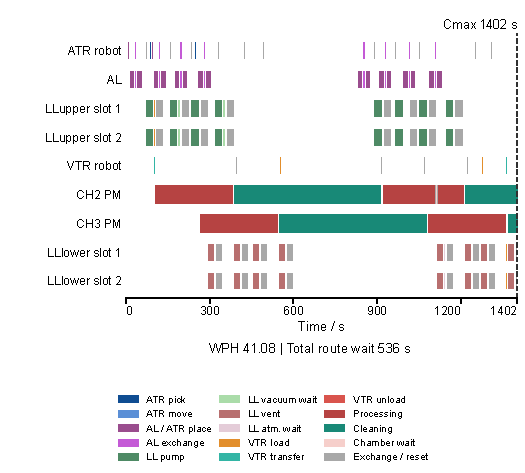
\includegraphics[width=0.825\textwidth]{fig_resource_gantt_cleanH3_w16_22_en_nature}
\caption{16-wafer pure $2\times2$ schedule at $H=3$: two internal and two terminal cleans, $C_{\max}=1402$~s, WPH = 41.08 wafers/h, and total route wait = 536~s. The horizon ends at product return; exchanges and waiting are shown separately.}
\label{fig:gantt-cleanH3-22-en}
\end{figure*}

\subsection{Equal-budget refinement of waiting and cadence}

Waiting-time constraints can propagate to manufacturing-system output and control performance \cite{lee2018waiting}. For the same 600-s total budget, the complete two-stage workflow assigns 540~s to the main solve and up to 60~s to refinement, whereas the one-stage control assigns all 600~s to the main solve. The measured instance means show that the two-stage workflow reduces total route wait, maximum wait, cadence coefficient of variation, and cadence deviation by 51.91\%, 68.89\%, 39.70\%, and 94.05\%, respectively. All four paired instance differences remain significant after Holm correction, demonstrating that the two-stage workflow markedly improves waiting and cadence quality under the same total budget.

The quadratic-objective control and the complete linear refinement both use the 540+up-to-60-s split. Linear refinement yields a cadence deviation of 22.04, 63.38\% below the quadratic profile's 60.18, and the matched difference remains significant after Holm correction ($p=0.0377$); total route wait, maximum wait, and cadence coefficient of variation are similar overall. The linear objective therefore reduces the measured cadence deviation under the same budget.


Table~\ref{tab:refinement-ablation-en} isolates the second stage and refinement objective, complementing the initialization ablation in Table~\ref{tab:spbs-en-new}.

\begin{table*}[!htbp]
\centering\footnotesize
\setlength{\tabcolsep}{3pt}
\caption{Ablation of second-stage refinement and objective form. Each configuration contains 20 instances and 500 runs under a 600-s total budget. Entries are instance-aggregated means; lower is better.}
\label{tab:refinement-ablation-en}
\begin{tabular}{ccccc}
\toprule
Configuration & Total wait (s) & Max. wait (s) & Cadence CV & Deviation (s)\\
\midrule
Full linear refinement & 2596.01 & 296.33 & 0.130 & 22.04\\
Quadratic refinement & 2469.47 & 293.27 & 0.134 & 60.18\\
Without stage two & 5398.60 & 952.57 & 0.216 & 370.41\\
\bottomrule
\end{tabular}
\end{table*}


\subsection{SPBS and structure-aware cut selection}

Table~\ref{tab:spbs-en-new} summarizes the paired SPBS study with 48 instances and ten paired seeds per instance. The timed comparison measures main-solver performance after offline SPBS construction. Relative to the no-start condition, precomputed SPBS increases incumbent availability from 51.67\% to 100\%, a gain of 48.33 percentage points (95\% interval $[34.58,62.29]$). Mean PDI falls from 27473.05 to 20278.78, a decrease of 7194.27 or 26.19\% (95\% interval $[5145.78,9317.61]$). Both paired differences remain significant after Holm correction ($p=2.55\times10^{-5}$ and $p=3.46\times10^{-8}$). Precomputed SPBS therefore improves feasible-schedule availability and primal--dual convergence during the subsequent solve.

\begin{table}[!htbp]
\centering
\footnotesize
\setlength{\tabcolsep}{3pt}
\caption{Effect of precomputed SPBS on time-limited MILP search; construction time is excluded. Each condition contains 48 instances and ten paired seeds per instance, totaling 480 runs.}
\label{tab:spbs-en-new}
\begin{tabular}{cccc}
\toprule
Metric & No start & SPBS & Observed change\\
\midrule
Incumbent rate (\%) & 51.67 & 100.00 & +48.33 points\\
Mean PDI & 27473.05 & 20278.78 & -26.19\%\\
\bottomrule
\end{tabular}
\end{table}

HEM-13D is the most direct learning baseline for the structure-aware cut selector. Both methods share SPBS, training instances, random seeds, candidate limits, hidden dimensions, and a 600-s solve budget, with 500 runs per method. Table~\ref{tab:all-methods} includes this prespecified direct comparison. Relative to HEM-13D, \method{} changes mean PDI from 16823.18 to 16585.70, mean solve time from 219.65 to 218.32~s, mean terminal gap from 127.24\% to 126.01\%, and proven-optimal rate from 62.4\% to 63.2\%. All 500 complete-method runs produce feasible schedules. After aggregating repeats over 20 manufacturing instances, all four paired mean-difference 95\% bootstrap intervals include zero and all Holm-adjusted $p$-values are 1.0. The observed means are close under the common SPBS condition; the paired tests provide the statistical context for these changes.



Table~\ref{tab:all-methods} adds default SCIP, validation-tuned adaptive cut scoring, and component ablations from the same frozen experiment. Nonlearning methods use five solver seeds per instance (100 runs each); each learned method additionally uses five training seeds (500 runs each). Configured SCIP has the highest observed optimal rate and lowest mean terminal gap, while the complete method has the lowest observed PDI and solve time. There is no consistent dominance across metrics.

\begin{table*}[t]
\centering\footnotesize
\caption{Complete frozen 2700-run comparison with common initial schedules and 600-s solver budgets. Values are means over 20 instance aggregates. Gap uses SCIP's terminal definition.}
\label{tab:all-methods}
\begin{tabular}{lrrrrr}\toprule
Method & Runs & PDI & Solve time (s) & Gap (\%) & Optimal (\%)\\\midrule
Configured SCIP & 100 & 16919.01 & 226.05 & 119.54 & 64.0 \\
Adaptive cut scoring & 100 & 16854.87 & 222.34 & 127.18 & 62.0 \\
HEM-13D & 500 & 16823.18 & 219.65 & 127.24 & 62.4 \\
23D features only & 500 & 16620.91 & 219.42 & 125.33 & 62.6 \\
HEM + beam & 500 & 16829.59 & 219.95 & 127.19 & 62.4 \\
Structure + greedy & 500 & 16598.11 & 218.44 & 126.03 & 63.2 \\
\method{} & 500 & 16585.70 & 218.32 & 126.01 & 63.2 \\
\bottomrule\end{tabular}\end{table*}

The comparison jointly evaluates role-aware representation, sequence decoding, and structural completion under common initialization and solver budgets, quantifying their effects on PDI, solution time, terminal gap, and proven-optimal rate with shared SPBS.

\subsection{Scale, recipe composition, and computational difficulty}

The factorial design contains $4\times5\times3=60$ wafer-count--recipe-composition--process-scale cells with five solver seeds per cell, for 300 runs. The results show a sharp transition. All 75 runs at both 8 and 16 wafers prove optimality, with mean PDI values of 28.13 and 1876.54 and mean solution times of 0.34 and 33.86~s. At 24 and 32 wafers, the proven-optimal rates fall to 36\% and 20\%, mean PDI rises to 31155.94 and 32959.89, and mean solution time reaches 408.55 and 433.20~s.

The prespecified PDI factorial model has $R^2=0.998$. Under the $1{:}1$ mixed recipe, the additional interaction coefficients at 24 and 32 wafers are 37729.48 and 40788.63, while the 95\% intervals for the process-scale main effect and all prespecified process-scale interactions include zero. Over the tested 0.9--1.1 process-scale range, computational difficulty is driven primarily by the interaction between batch size and mixed-flow composition, with a comparatively small process-scale effect.



\subsection{Operation under parameter perturbations}

Prior CT studies show that cleaning actions and their triggering conditions alter robot-task sequences, cycle time, and wafer delay \cite{yu2020delay,li2022conditioncleaning}. The one-factor sensitivity study therefore covers eight prescribed perturbations of transport, processing, cleaning interval, and vacuum-domain dummy inventory, for 80 runs. Every run returns a solver-checked feasible schedule and 20 runs prove optimality; scenario mean PDI ranges from 28899.41 to 42478.32. A longer cleaning interval gives the lowest mean PDI and slower transport the highest, describing the variation in search performance across the tested parameter settings.

\subsection{Feasible-schedule delivery under distribution shift}

The distribution-shift suite enlarges batches to 40--64 wafers and changes mixed-flow composition, producing 729 runs across all compared methods over nine shifted manufacturing scenarios, including 135 runs of the complete method. This experiment evaluates schedule availability and search performance under changes in scale and composition. All 729 runs return an incumbent that passes SCIP and independent post-solve checks. The shared SPBS--MILP--SCIP chain therefore continues to output a validated resource-action schedule over the tested changes in scale and recipe composition. The proven-optimal rate is 0\%. The complete method has mean PDI 73919.15, compared with 73670.99 for default SCIP and 70915.54 for adaptive cut scoring. Feasible-schedule availability is 100\% across this suite, while adaptive cut scoring has the lowest observed mean PDI.

\subsection{Discussion of mode selection and computational performance}

Mode preference depends on where cleaning occurs within a finite batch. Internal cleaning delays subsequent chains, whereas terminal cleaning affects the product-return objective differently. Mixed operation is preferred at $H=4$ for 16 wafers and at $H=6$ for 24 wafers. Thus, single-cycle processing capability or cleaning interval alone does not determine the preferred finite-batch mode; lot size and complete-chain layout also matter.

Mode preference can be established directly by comparing a feasible upper bound with competing lower bounds. For 24 wafers at $H=7$--10, the pure $2\times2$ upper bound of 1237~s lies below both competing optima, establishing its preference among the compared layouts. Mode comparisons determine process choices for a given lot size and cleaning interval, while equal-budget algorithm comparisons quantify search performance.

The solver components address different schedule-performance measures. Precomputed SPBS improves feasible-schedule availability in subsequent time-limited search, and two-stage refinement improves waiting and cadence. With common SPBS, the complete cut selector and HEM have close observed mean metrics. Scale-extension experiments achieve 100\% feasible-schedule availability, and adaptive scoring yields the lowest observed mean PDI. These results quantify schedule availability, timing quality, and bound convergence separately. The parameter-perturbation study reoptimizes deterministic instances and does not test execution under random disturbances. A feasible returned schedule satisfies the modeled constraints; this does not prove closed-loop stability, recovery from breakdowns, or a hard online response-time guarantee.

\section{Conclusions}
The proposed two-stage MILP coordinates product and reusable dummy flows, chamber occupancy, cleaning and shared-resource timing for finite batches. Under prescribed qualified recipes and pair layouts, the preferred mode depends on lot size and cleaning-induced chain segmentation. Chained processing reaches 898~s for a 16-wafer lot without activated cleaning, compared with 944~s for parallel processing. Valid upper and lower bounds establish the reported mode choices without treating a time limit as an infeasibility proof.

The frozen computational evidence supports the scheduling value of precomputed feasible starts and equal-budget waiting/cadence refinement. It does not establish statistical superiority of the complete cut selector over HEM, nor a universal out-of-distribution advantage. Further work should measure initialization-inclusive decision latency, relax prescribed pair placement, and validate disturbance handling and recipe qualification on physical equipment.

\section*{Acknowledgment}
OpenAI ChatGPT and Codex assisted with language revision and Chinese--English translation throughout the manuscript, the restructuring of the Abstract, Note to Practitioners, Introduction and Discussion, LaTeX preparation, and development/debugging of the numerical solution and visualization code described in Sections~III--IV. Reported numerical results are retained from solver experiments; no new experimental outcomes were generated for this manuscript conversion.

\bibliographystyle{IEEEtran}
\bibliography{references}
\end{document}
